%% Präsentation CUDA Semina


\documentclass[compress,t]{beamer}
%\documentclass[draft,compress,notes,t]{beamer}
%\documentclass[compress,notes=only,t]{beamer}
%\documentclass[compress,handout,t]{beamer}
%\documentclass{article}
%\usepackage{pgfpages}
\usetheme{Dresden}
\usecolortheme{beaver}
\beamertemplatenavigationsymbolsempty
\setbeamertemplate{footline}[frame number]
%\usepackage{beamerthemeshadow}
%\beamersetuncovermixins{\opaqueness<1>{25}}{\opaqueness<2->{15}}


%\usepackage{beamerarticle}
\usepackage[ngerman]{babel}
\usepackage[utf8]{inputenc}
\usepackage{amsmath,amsfonts,amssymb}
\usepackage[linesnumbered]{algorithm2e}
\usepackage{float}
\setbeamertemplate{section in toc}[default]


\title{Sorting}
\subtitle{Effiziente Sortieralgorithmen für Manycore GPUs}
\author[A. Groß]{André Groß}
\institute{Institut für Informatik\\ Johannes Gutenberg Universität Mainz}
\date{\today}
%\logo{
\includegraphics[scale=.08]{logo_schriftzug}}
\titlegraphic{
\includegraphics[scale=.3]{logo}}

\AtBeginSection[]{%
  \begin{frame}
    \frametitle{Inhaltsverzeichnis}
	\setcounter{tocdepth}{2}
    \tableofcontents[sectionstyle=show/shaded,subsectionstyle=hide/show/hide]
    \hfill
  \end{frame}
  \addtocounter{framenumber}{-1}
}




\begin{document}
\frame{
	\titlepage
\note{Titel, dann Inhalt...\\ \tiny \setcounter{tocdepth}{2} \tableofcontents \normalsize} 
}
\frame{
	\frametitle{Inhaltsverzeichnis}
	\setcounter{tocdepth}{1}
	\tableofcontents[pausesections]
}


\section{Einführung}
\frame{\frametitle{Einführung}
\begin{itemize}
	\item<1->Basis vieler Algorithmen \note<4>[item]{Viele Algorithmen benötigen effiziente Sortieralgorithmen} 
	\item<2->Datenbanksysteme \note<4>[item]{Abfragen Sortieren} 
	\item<3->Computer Graphik \note<4>[item]{Sichtbarkeitsproblem} 
	\item<4->Geographische Informationssysteme \note<4>[item]{Viele Algorithmen benötigen effiziente Sortieralgorithmen} 
\end{itemize} 
}

\subsection{Stichwörter}
\frame{\frametitle{Stichwörter}
\begin{itemize}
	\item<1->Stabil und Instabil
		\note<4>[item]{}
	\item<2->Direkt und Indirekt
		\note<4>[item]{}
	\item<3->In-place und Out-of-place ("'in situ"' / "'ex situ"')
		\note<4>[item]{}
	\item<4->Vergleichsbasiert
		\note<4>[item]{}
\end{itemize} 
}



\subsection{Ausgewählte Algorithmen}
\frame{\frametitle{Ausgewählte Algorithmen}
\begin{itemize}
	\item<1->t
		\note<4>[item]{}
	\item<2->t
		\note<4>[item]{}
	\item<3->t
		\note<4>[item]{}
	\item<4->t
		\note<4>[item]{}
\end{itemize} 
}



\subsection{Probleme der Parallelisierung}
\subsubsection{Effizienz}
\frame{\frametitle{Probleme der Parallelisierung}
\framesubtitle{Effizienz}
\begin{itemize}
	\item<1->Cache line size
		\note<4>[item]{}
	\item<2->Execution divergence
		\note<4>[item]{nicht beim warp}
	\item<3->Shared memory
		\note<4>[item]{}
	\item<4->Use of gather and scatter
		\note<4>[item]{}
	\item<5->Consecutive access (coalesce)
\end{itemize} 
}
\subsubsection{Design}
\frame{\frametitle{Probleme der Parallelisierung}
\framesubtitle{Design}
\begin{itemize}
	\item<1->Divide and Conquer
		\note<4>[item]{}
	\item<2-> $p$ thread blocks of $t$ threads each
		\note<4>[item]{nicht beim warp}
	\item<3->Focus on decomposition between blocks
		\note<4>[item]{}
	\item<4->Barriers
		\note<4>[item]{}
	\item<5->Consecutive access (coalesce)
\end{itemize} 
}



\section{Radix Sort}
\frame{\frametitle{Radix Sort}
\begin{itemize}
	\item<1->Alt und am besten verstanden
		\note<6>[item]{}
	\item<2->Meist die effizienteste Wahl
		\note<6>[item]{Für kleine Schlüssel}
	\item<3->Und immer noch
		\note<6>[item]{Paper Thouti, Sathe 2012}
	\item<4->Stabil aber out-of-place
		\note<6>[item]{}
	\item<5->Basiert auf Counting oder Bucket- Sort
		\note<6>[item]{}
	\item<6->Laufzeit liegt in $\mathcal O(n)$
		\note<6>[item]{}
\end{itemize} 
}



\subsection{Sequentiell}
\frame{\frametitle{Sequentiell}
\framesubtitle{Wie Radix Sort sequentiell funktioniert}
\begin{itemize}
	\item In die Eimer
	\item und wieder hinaus
\end{itemize}
\begin{table}[ht!]\pause
\begin{tabular}{ccccccccc}
$A$&$5|101$&$7|111$&$2|010$&$1|001$&$4|100$&$6|110$&$3|011$&$0|000$\pause\\
$B[0]$&$2|01\color{red}{0}$&$4|10\color{red}{0}$&$6|11\color{red}{0}$&$0|00\color{red}{0}$&&&&\\
$B[1]$&$5|10\color{red}{1}$&$7|11\color{red}{1}$&$1|00\color{red}{1}$&$3|01\color{red}{1}$&&&&\pause\\  \hline
$A$&$2|010$&$4|100$&$6|110$&$0|000$&$5|101$&$7|111$&$1|001$&$3|011$\pause\\
$B[0]$&$4|100$&$0|000$&$5|101$&$1|001$&&&&\\
$B[1]$&$2|010$&$6|110$&$7|111$&$3|011$&&&&\pause\\\hline
$A$&$4|100$&$0|000$&$5|101$&$1|001$&$2|010$&$6|110$&$7|111$&$3|011$\\
$B[0]$&$0|000$&$1|001$&$2|010$&$3|011$&&&&\\
$B[1]$&$4|100$&$5|101$&$6|110$&$7|111$&&&&\pause\\\hline
$A$&$0|000$&$1|001$&$2|010$&$3|011$&$4|100$&$5|101$&$6|110$&$7|111$\\
\end{tabular}
\end{table}
}



\subsection{Idee}
\frame{\frametitle{Idee}
\begin{itemize}
	\item<1->Kacheln der Sequenz
		\note<5>[item]{}
	\item<2->Effiziente Nutzung der Speicherbandbreite\\
		\note<5>[item]{Für kleine Schlüssel}
		\begin{enumerate}
			\item wenige Scatter zu Global Mem.
			\item maximale Kohärenz der Scatter
		\end{enumerate}
	\item<3->1:
		\note<5>[item]{}
	\item<4->2:
		\note<5>[item]{}
	\item<5->Unterteilung in vier Phasen
		\note<5>[item]{}
\end{itemize} 
}



\subsection{Der Counting Sort}
\frame{\frametitle{Der Counting Sort\footnote{Quelle: Wikipedia}}
\begin{columns}
\begin{column}{5cm}
\begin{enumerate}
	\item<1-4> Histogramm
		\note<5>[item]{}
	\item<2-4> Präfixsumme
		\note<5>[item]{}
	\item<3-4> Der Sortiervorgang
		\note<5>[item]{}
\end{enumerate}
\uncover<4->{}
\vspace{3cm} 
\end{column}
\begin{column}{5cm}\scriptsize
\begin{figure}
\begin{algorithm}[H]
\uncover<1->{\KwData{$I\gets input$,$m\gets maxKeyValue$}
$H \gets \emptyset$\;
\ForAll{$i \in I$}{
	$H[i.key]++$\;
}}
\uncover<2->{$count=0$\;
\For{$i=1; i<=m; i++$}{
	$H[i] += H[i-1]$\;
}}
\uncover<3->{$O\gets\emptyset $\;
\ForAll{$i \in I$}{
	$O[H[i.key]]=i$\;
	$H[i.key]] --$\;
}}
\end{algorithm}
\end{figure}
\end{column}
\end{columns}
}



\subsection{Die Phasen}
\frame{\frametitle{Die Phasen}
\begin{columns}
\begin{column}{5cm}
\begin{enumerate}
	\item<1-5> Tiles werden in Shared geladen und sortiert
		\note<5>[item]{}
	\item<2-5> Histogramm wird errechnet und zusammen mit den Tiles zu Global zurück geschrieben
		\note<5>[item]{}
	\item<3-5> Präfixsumme über Histogramm für globalen Offset
		\note<5>[item]{}
	\item<4-5> Kopieren der Objekte zur korrekten Ausgabeposition
		\note<5>[item]{}
\end{enumerate}
\vspace{3cm} 
\end{column}
\begin{column}{5cm}\scriptsize
\begin{figure}
\begin{algorithm}[H]
\uncover<1->{\KwData{$I\gets input$,$m\gets maxKeyValue$}}
\uncover<2->{
$H \gets \emptyset$\;
\ForAll{$i \in I$}{
	$H[i.key]++$\;
}}
\uncover<3->{$count=0$\;
\For{$i=1; i<=m; i++$}{
	$H[i] += H[i-1]$\;
}}
\uncover<4->{$O\gets\emptyset $\;
\ForAll{$i \in I$}{
	$O[H[i.key]]=i$\;
	$H[i.key]] --$\;
}}
\end{algorithm}
\end{figure}
\end{column}
\end{columns}
}



\subsection{Optimierung}
\frame{\frametitle{Optimierung}
\begin{itemize}
	\item<1->Viele Elemente pro Tread
		\note<6>[item]{}
	\item<2->Viel unabhängige serielle Arbeit
		\note<6>[item]{}
	\item<3->Die Wahl von $b$
		\begin{itemize}
			\item<4-> $b>>:$ schlechtere Kohärenz
			\item<5-> $b<<:$ mehr Scatter
		\end{itemize}
	\item<6->
		\note<6>[item]{}
\end{itemize} 
}



\section{Merge Sort}
\frame{\frametitle{Merge Sort}
\begin{itemize}
	\item<1->Vergleichsbasiert
		\note<6>[item]{}
	\item<2->Stabil aber out-of-place
		\note<6>[item]{}
	\item<3->Laufzeit liegt in $\mathcal O(n\log n)$
		\note<6>[item]{}
	\item<4->Bevorzugt für externes Sortieren
		\note<6>[item]{}
	\item<5->Prozessoren mit wenig Speicher
		\note<6>[item]{Global 4GB, Shared 16K}
	\item<6->
		\note<6>[item]{}
\end{itemize} 
}



\subsection{Sequentiell}
\frame{\frametitle{Sequentiell}
\begin{columns}
\begin{column}{5cm}
\begin{figure}
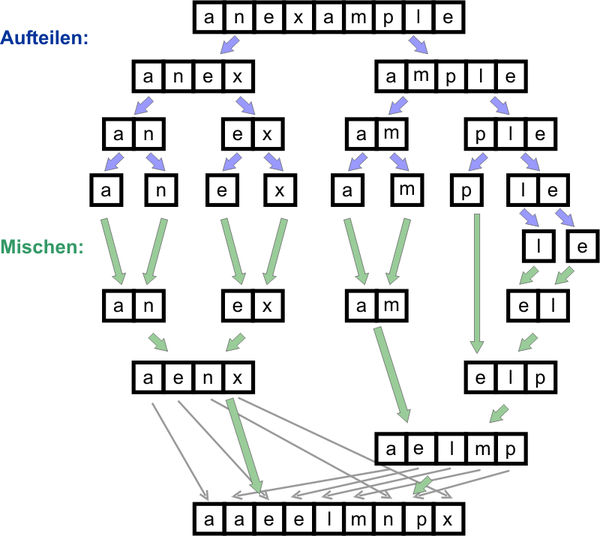
\includegraphics{mergesort}
\caption{Merge-Sort\footnote{Quelle: Wikipedia}}
\end{figure}
\vspace{3cm} 
\end{column}
\begin{column}{5cm}\scriptsize
\end{column}
\end{columns}
}



\subsection{Idee}
\frame{\frametitle{}
}



\subsection{Probleme}
\frame{\frametitle{}
}



\subsection{Verbesserungen}
\frame{\frametitle{}
}



\section{Schluss}
\frame{\frametitle{}
}



\subsection{Alternativen}
\frame{\frametitle{}
}



\subsection{Fazit}
\frame{\frametitle{}
}



{ % black page
\setbeamercolor{background canvas}{bg=black}
\frame[plain]{}
} 
\end{document}
